% Unified-model design space — TikZ source. Compiles to a tight standalone PDF
% (pdflatex figures/design-space.tex), which `book-scaffold build-figures`
% converts to public/figures/design-space.svg.
%
% Three designs that share the SAME modality-blind body: merged single-stream,
% two-path (separate connector + head), and continuous-in/discrete-out hybrid.
\documentclass[tikz,border=3pt]{standalone}
\usepackage{amsmath}
\usepackage{amssymb}
\usepackage{tikz}
\usetikzlibrary{positioning,arrows.meta,calc}
\begin{document}
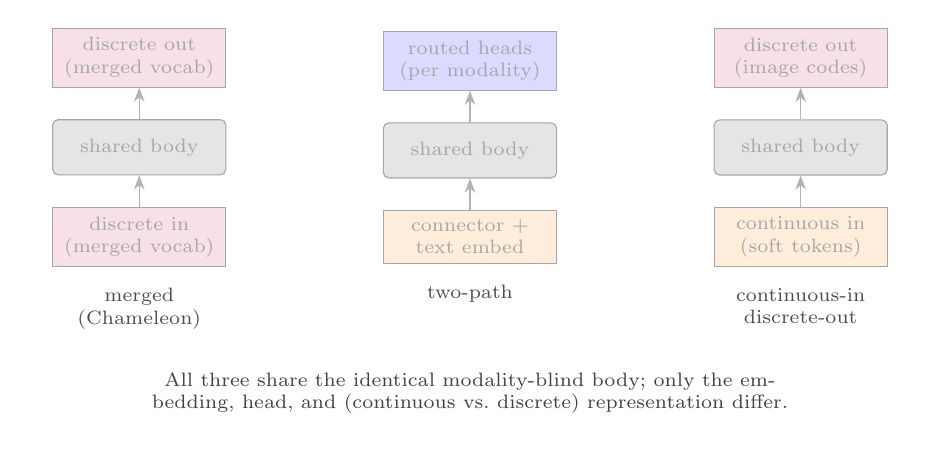
\begin{tikzpicture}[
    font=\small,
    body/.style={draw, gray!70, rounded corners=2pt, fill=black!10,
                 minimum width=22mm, minimum height=7mm, align=center,
                 font=\scriptsize},
    io/.style={draw, gray!70, minimum width=22mm, minimum height=6mm,
               align=center, font=\scriptsize},
    op/.style={->, >={Stealth[length=1.8mm]}, gray!60},
  ]
  % --- Design 1: merged single-stream ---
  \begin{scope}
    \node[io, fill=purple!12] (in1) {discrete in\\(merged vocab)};
    \node[body, above=4mm of in1] (b1) {shared body};
    \node[io, fill=purple!12, above=4mm of b1] (out1) {discrete out\\(merged vocab)};
    \draw[op] (in1) -- (b1); \draw[op] (b1) -- (out1);
    \node[below=1.5mm of in1, font=\scriptsize, text=black!70, align=center]
      {merged\\(Chameleon)};
  \end{scope}
  % --- Design 2: two-path ---
  \begin{scope}[xshift=42mm]
    \node[io, fill=orange!14] (in2) {connector +\\text embed};
    \node[body, above=4mm of in2] (b2) {shared body};
    \node[io, fill=blue!14, above=4mm of b2] (out2) {routed heads\\(per modality)};
    \draw[op] (in2) -- (b2); \draw[op] (b2) -- (out2);
    \node[below=1.5mm of in2, font=\scriptsize, text=black!70, align=center]
      {two-path};
  \end{scope}
  % --- Design 3: continuous-in / discrete-out ---
  \begin{scope}[xshift=84mm]
    \node[io, fill=orange!14] (in3) {continuous in\\(soft tokens)};
    \node[body, above=4mm of in3] (b3) {shared body};
    \node[io, fill=purple!12, above=4mm of b3] (out3) {discrete out\\(image codes)};
    \draw[op] (in3) -- (b3); \draw[op] (b3) -- (out3);
    \node[below=1.5mm of in3, font=\scriptsize, text=black!70, align=center]
      {continuous-in\\discrete-out};
  \end{scope}

  \node[below, align=center, text width=11cm, font=\scriptsize, text=black!75]
    at (42mm,-1.6)
    {All three share the identical modality-blind body; only the embedding, head,
     and (continuous vs.\ discrete) representation differ.};
\end{tikzpicture}
\end{document}
